\chapter{Results and Conclusions}
\label{chap:six}

In this chapter, we illustrate the performance of our fusion ordering in a real-world multi-robot dataset \cite{radish} recorded at AP hill, Virginia. For our datasets, we use a canonical scan-matcher \cite{csmicp} that remembers a short history of scans corresponding to the key frames, fits contours to the data, and for a new scan, finds a globally optimal alignment within a given search region. The canonical scan-matcher performs another least-squares optimization that requires an initial guess about the relative transform between the scans. The relative odometry measurement coming from the poses corresponding to those scans is used as an initial guess. Larger key frame sizes are also problematic as the scan ranges vary significantly due to seeing an altogether different structure of the environment. This leads to a large uncertainty in the estimate of the relative transform. It is also difficult to provide a good initial guess for large key frame sizes as the corresponding odometry transform is likely to be drifted. In our results, we project the raw laser scans from the optimized trajectory of every robot instead of occupancy grid as the occupancy grid can sometime hide the inaccuracies in the map, such as duplication of a wall. However, we also show the occupancy grid to comply with the usual practise in the SLAM literature.

\section{AP Hill Multi-robot Dataset}
The publicly available AP hill multi-robot dataset \cite{radish} is recorded using 4 mobile robots with significant overlap in their trajectories. The robots travel different paths covering different blocks in the building. Each robot is equipped with an odometer, a laser range finder, an inertial measurement unit and a camera. Encounter information is also provided along with the dataset. According to the dataset, all the robots start at nearly the same position, and hence the number of encounters in the later stages are less in number. In general, we increase the number of encounters by performing multi-channel fiducial detection (see Chapter \label{chap:five}) using the data obtained from the camera mounted on the robots. Getting a good map of the environment is an engineering task that requires tuning of several optimization parameters and those related to different measurement models. In this section, we will describe the numerical values that are used for different sensor models and ISAM2 algorithm in GTSAM optimizer \cite{gtsamhandson}. We will then present the timing analysis for using the fusion ordering for the combined graphs during every encounter. Finally the map alignment that is obtained by adding the relative transform between the trajectories as an estimation variable is displayed. 

\subsection{Tuning the Sensor Models and GTSAM Optimizer}
Getting the optimizer up and running to provide consistent and repeatable mapping results is generally preceded by developing accurate sensor models. The AP hill multi-robot dataset contains raw wheel encoder data, dead reckoning odometry data, laser range data, IMU data and the camera feed. The raw wheel encoder data is processed using a velocity motion model given in Appendix \ref{appendix:one}. The laser range data is used by the scan-matching module, also described in Appendix \ref{appendix:one}, to convert it into pose constraint. The IMU data is also treated in a similar manner to make it as a pose factor. Apart from the velocity model factors the dead reckoning odometry data is also used. Thus, all the pose variables are constrained by a minimum of four types of factors. In addition to the fiducials on top of every robot the environment also contains fiducials that serve as the landmarks. These fiducial and encounter information in the dataset are converted into a constraint between the poses and the landmarks/other robots. We also detect the same on the camera feed to further constrain the variables and over-determine the system. 
\paragraph{}
All these sensor models are accurate to a level that depends on the amount of uncertainty it introduces in the system. This level of uncertainty is captured by the covariance matrix that measures the joint variability of different random variables measured by the model. In other words, the sensor that is less accurate has a larger covariance. In many cases, they are provided by the sensor manufacturer. They can be used as a starting point and can then be tuned based on performance. For encoders like odometry, the error accrued is larger for larger sampling times. For such sensors, the covariance is tuned for unit time and scaled accordingly based on the time between different samples. In case of fiducial markers, the center of the detected fiducial is taken as the landmark position and therefore its covariance is also defined in terms of $x$, $y$ and $\theta$. The encounter covariance works same as the fiducial covariance as they are also fiducial markers attached to the robot. A loop closure introduces a correlation between the current pose and a previous pose occurred long back in time from which the current portion of the environment is observed. So a loop closure is also represented by a factor between robot poses at fairly farther time instants. The IMU model also estimates the relative transformation between robot poses and contains the same variables over which the covariance is represented. The tuned values of model covariance that are finally used for mapping are presented in Table \ref{table:cov}.
% Please add the following required packages to your document preamble:
% \usepackage{multirow}
% \usepackage{graphicx}
\begin{table}[]
\centering
\caption{Tuned covariance values of various sensor models used for mapping. These values are used to calculate the Bhattacharyya distance in the least-squares problem formulated in Chapter \ref{chap:two}. The covariance matrix for $n$ variables contain $n^2$ terms, but we tune the values only across the main diagonal (variance of each variable).}
\label{table:cov}
\resizebox{\textwidth}{!}{%
\begin{tabular}{|l|l|l|l|l|l|l|l|l|l|l|l|l|}
\hline
\multirow{2}{*}{Sensor Model} & \multicolumn{3}{l|}{robot 1} & \multicolumn{3}{l|}{robot 2} & \multicolumn{3}{l|}{robot 3} & \multicolumn{3}{l|}{robot 4} \\ \cline{2-13} 
                              & x (m) & y (m) & $\theta$ (rad) & x (m) & y (m) & $\theta$ (rad) & x (m) & y (m) & $\theta$ (rad) & x (m) & y (m) & $\theta$ (rad) \\ \hline
Velocity motion model         & 0.05  & 0.02  & 0.2          & 0.055 & 0.02  & 0.2          & 0.05  & 0.02  & 0.2          & 0.02  & 0.05  & 0.2          \\ \hline
Odometry model                & 0.04  & 0.02  & 0.5          & 0.04  & 0.03  & 0.5          & 0.05  & 0.022 & 0.1          & 0.023 & 0.013 & 0.2          \\ \hline
Landmark pose                 & 0.02  & 0.01  & 0.01         & 0.02  & 0.01  & 0.01         & 0.02  & 0.02  & 0.001        & 0.02  & 0.01  & 0.01         \\ \hline
IMU model                     & 0.02  & 0.01  & 0.05         & 0.02  & 0.01  & 0.05         & 0.01  & 0.01  & 0.001        & 0.01  & 0.01  & 0.01         \\ \hline
Loop closure factor           & 0.02  & 0.02  & 0.1          & 0.01  & 0.01  & 0.1          & 0.01  & 0.01  & 0.001        & 0.02  & 0.02  & 0.1          \\ \hline
Robot-robot encounter         & 0.01  & 0.01  & 0.2          & 0.01  & 0.01  & 0.02         & 0.01  & 0.01  & 0.2          & 0.01  & 0.01  & 0.2          \\ \hline
\end{tabular}%
}
\end{table}

\subsection{Global Map Alignment}
The global consistency in aligning the maps from multiple robots is achieved by using the ``global nails" introduced in Chapter \ref{chap:four}. The prior over the starting pose for the robots are initialized arbitrarily with minimum effort on tuning. Providing a prior over the starting pose is trivial for a single robot case as all the sensor measurements are locally consistent and the global alignment can be adjusted at any point in time. However, in a multi-robot scenario or in a lifelong and repeated mapping of the same environment, the prior over the initial pose should be known with certainty to fuse the common variables of estimation. To overcome this, an acceptable level of uncertain prior is tuned and improved via optimization with the global nail. The global nail corresponding to a particular robot is introduced only on its first encounter. A prior over the global nail of atleast one of the robots should be provided to prevent the entire system from having a gauge freedom. The alignment of the projected laser scan with and without using the global nail to calculate the relative transformation is shown in Figure \ref{fig:wo_align} and \ref{fig:w_align}. Each robot's trajectory is plotted with a unique color and its corresponding laser scan is depicted using a faded variant of the same color. The estimated final value of global nail variables are shown in the third column of the Table \ref{table:global_nail}. The second column lists the tuned values of all these variables and are used as an initial guess for optimization. The variable $T_r^G$ refers to the transformation from the starting point of robot $r$ to the global frame. 

\begin{table}[]
\centering
\caption{Tuned values for the prior over initial pose of every robot and the values obtained by optimization using the global nail.}
\label{table:global_nail}
\begin{tabular}{|l|l|l|l|l|l|l|}
\hline
\multirow{3}{*}{} & \multicolumn{6}{l|}{Value of relative pose graph transform} \\ \cline{2-7} 
 & \multicolumn{3}{l|}{w/o global nail} & \multicolumn{3}{l|}{w/ global nail} \\ \cline{2-7} 
 & x & y & $\theta$ & x & y & $\theta$ \\ \hline
$T_G^1$ & 0 & 0 & 0 & 0.401 & 0.299 & 0 \\ \hline
$T_G^2$ & -1.22 & 0.61 & 0 & -1.22 & 0.61 & 0 \\ \hline
$T_G^3$ & -2.44 & 0 & 0.1 & -2.44 & 0 & 0 \\ \hline
$T_G^4$ & -3.66 & 0.61 & 0 & -4.66 & 0.36 & 0 \\ \hline
\end{tabular}
\end{table}

\begin{figure}[H]
\centering
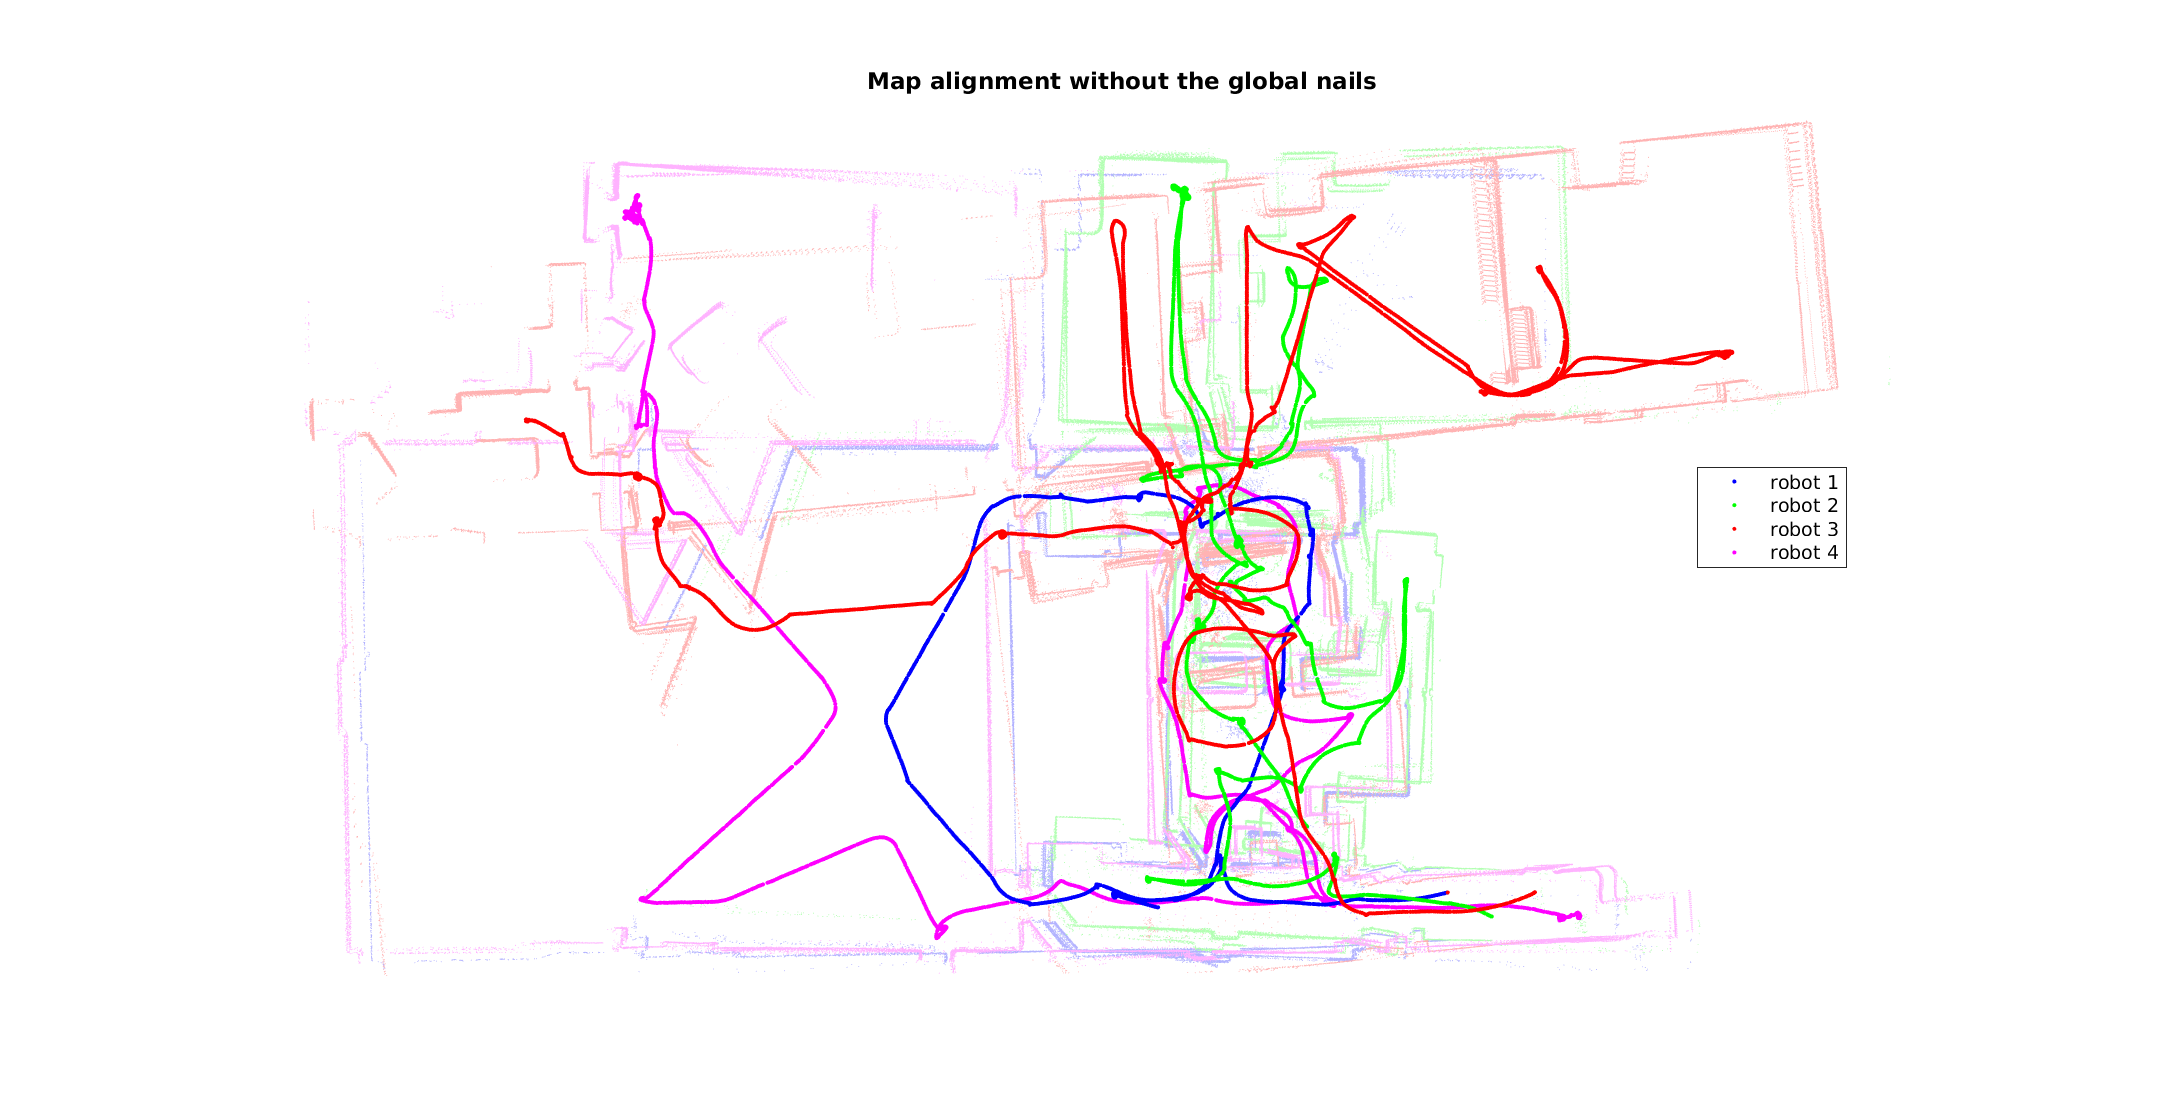
\includegraphics[width=\textwidth]{Chapters/figures6/without_map_alignment}
\caption{Overlay of laser scan projections from the smoothed trajectory of different robots. The optimization is done without the inter-robot relative pose transform constraint called ``global nail". It can be seen that, even after sufficient tuning of the prior over initial variables based on the map estimates at the early stages, we were not able achieve a total alignment.}
\label{fig:wo_align}
\end{figure}
\begin{figure}[H]
\centering
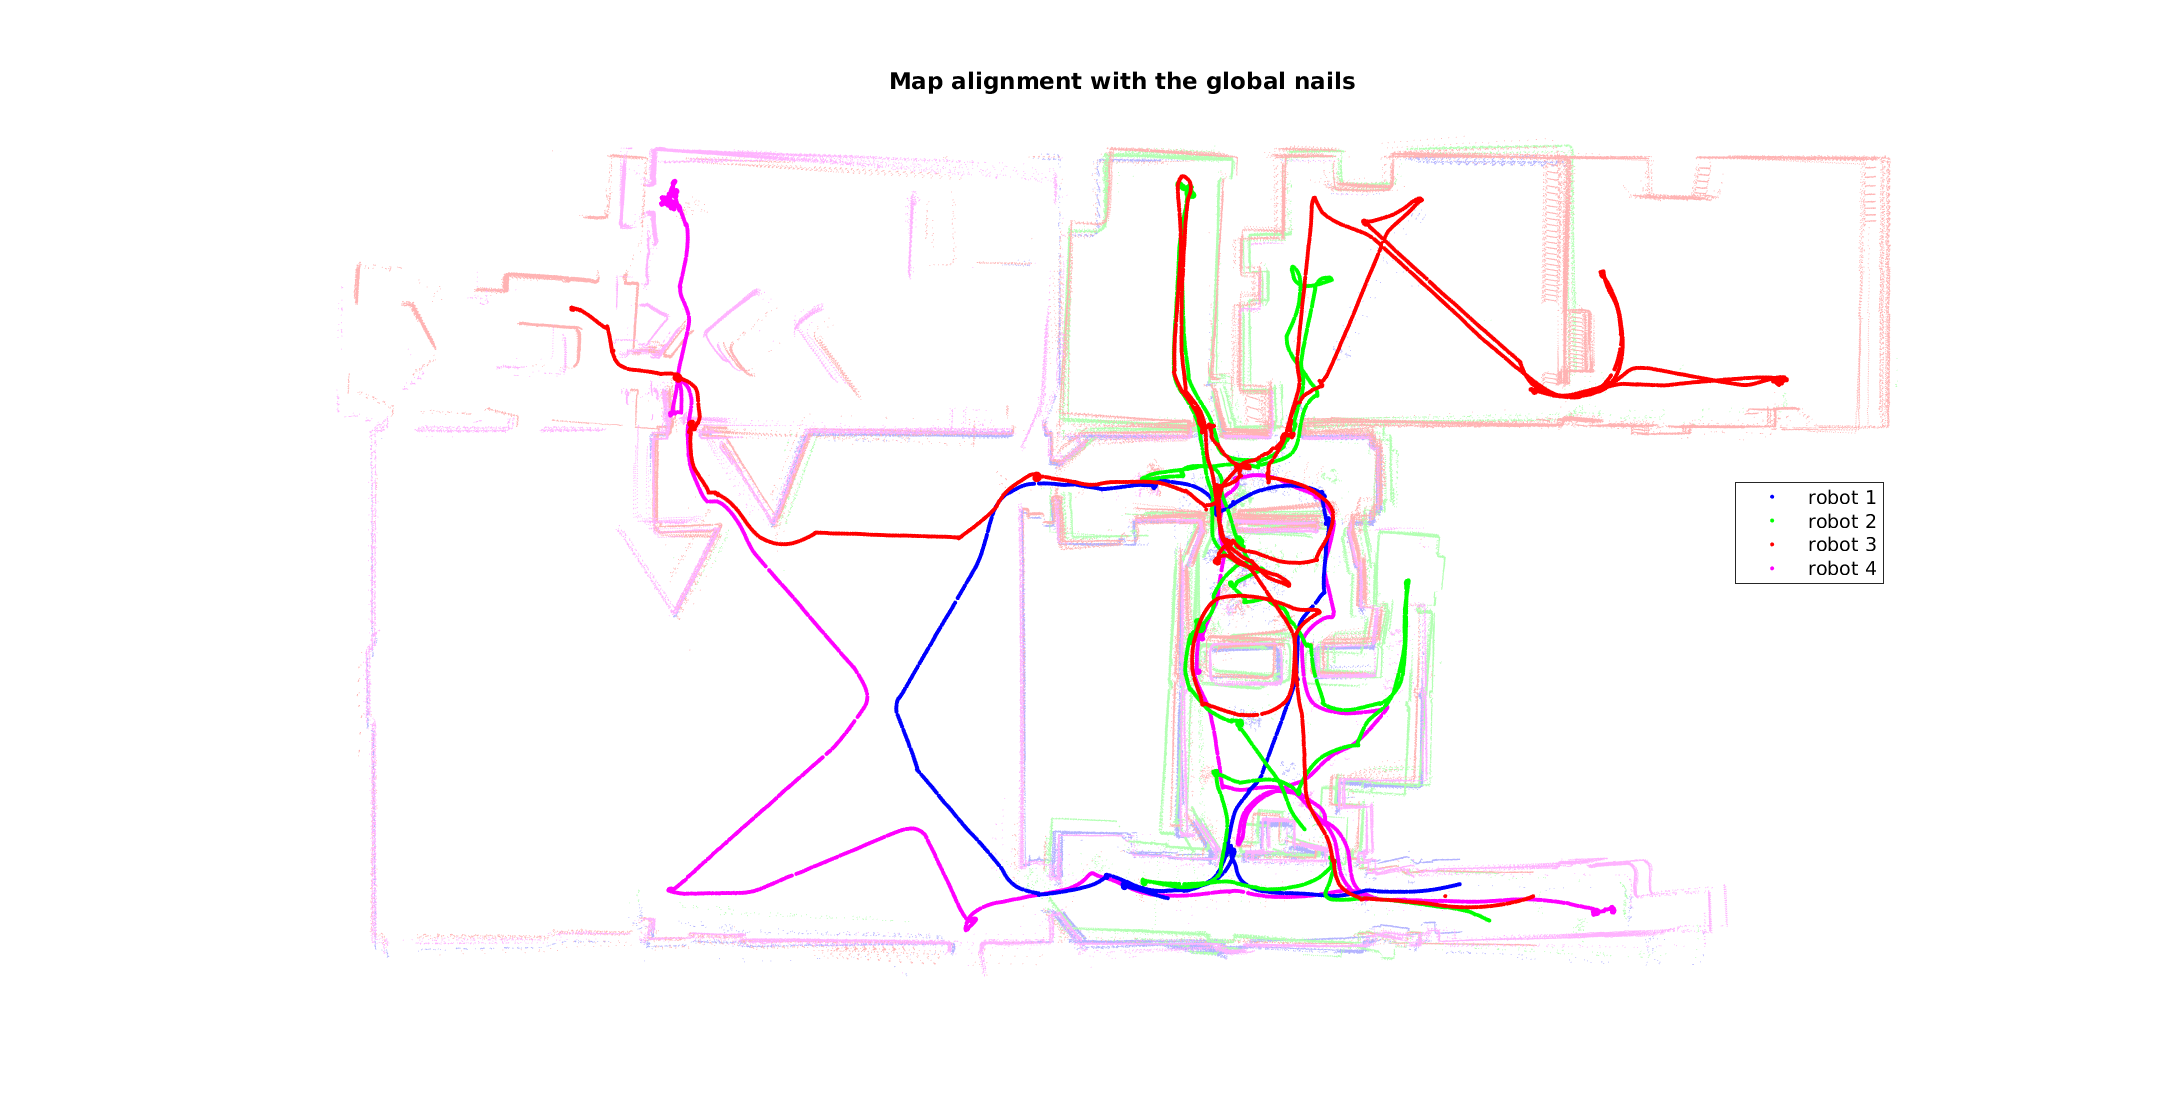
\includegraphics[width=\textwidth]{Chapters/figures6/with_map_alignment}
\caption{Overlay of laser scan projections from the smoothed trajectory of different robots. By adding the global nail constraints the relative transform between the robot trajectories are estimated accurates giving us a very good map alignment.}
\label{fig:w_align}
\end{figure}

\subsection{Fusion ordering vs. COLAMD ordering}
Whenever there is a direct or an indirect encounter, a factor between already existing common variable(s) or a new common variable is added. This leads to fusing the corresponding Bayes trees and marginalizing out the respective robot's variables. These marginals are then added as a strong prior to each robot's factor graph. The marginals of the ``global nail" variables from the fused graph are also added as a prior to the individual robot's factor graph that contains these ``global nail" variables. In practise, the graphs are fused for every few encounters and not every encounter. The performance is compared in terms of time it takes to calculate both these orderings. This ordering time does not include the time it takes to factorize the ordered measurement Jacobian. However, as fusion ordering leaves the Jacobian in a format explained in \cite{parallelqr} it can be subjected to parallel QR factorization. As a result, the time taken for factorization could be equal or lesser than using the COLAMD ordering. This phenomenon was already discussed while demonstrating the timing analysis on SuiteSparse dataset in Chapter \ref{chap:three}. 
\paragraph{}
The time taken for either of the ordering schemes are shown graphically using an encounter map in Figure \ref{fig:encounter_colamd} and \ref{fig:encounter_fusion}. The encounter maps contain the smoothed, centralized and final trajectory of all the robots using the combined information during every encounter. A line segment connecting the two trajectories indicate a robot-robot encounter from those poses at its endpoint. The color of the line segment reflects the time taken to compute the COLAMD ordering in Figure \ref{fig:encounter_colamd} or the fused ordering in Figure \ref{fig:encounter_fusion}. The color code reference is displayed with a color-bar on the right side of the encounter maps. The dataset contains roughly around 6000 direct robot-robot encounters and 300 indirect robot-landmark-robot encounters. It can clearly be observed that the color of the line segment for fusion ordering, when compared with that of nearly the same line segment for COLAMD ordering lies well below in the color-bar. This implies that the fusion ordering is faster in terms of computation than the COLAMD ordering. A more straightforward plot comparing the time taken by both these orderings is presented in Figure \ref{fig:fusion_vs_colamd}. Figure \ref{fig:fusion_vs_colamd} also includes the time taken for ordering the fused graph from indirect encounters.

\begin{figure}
\centering
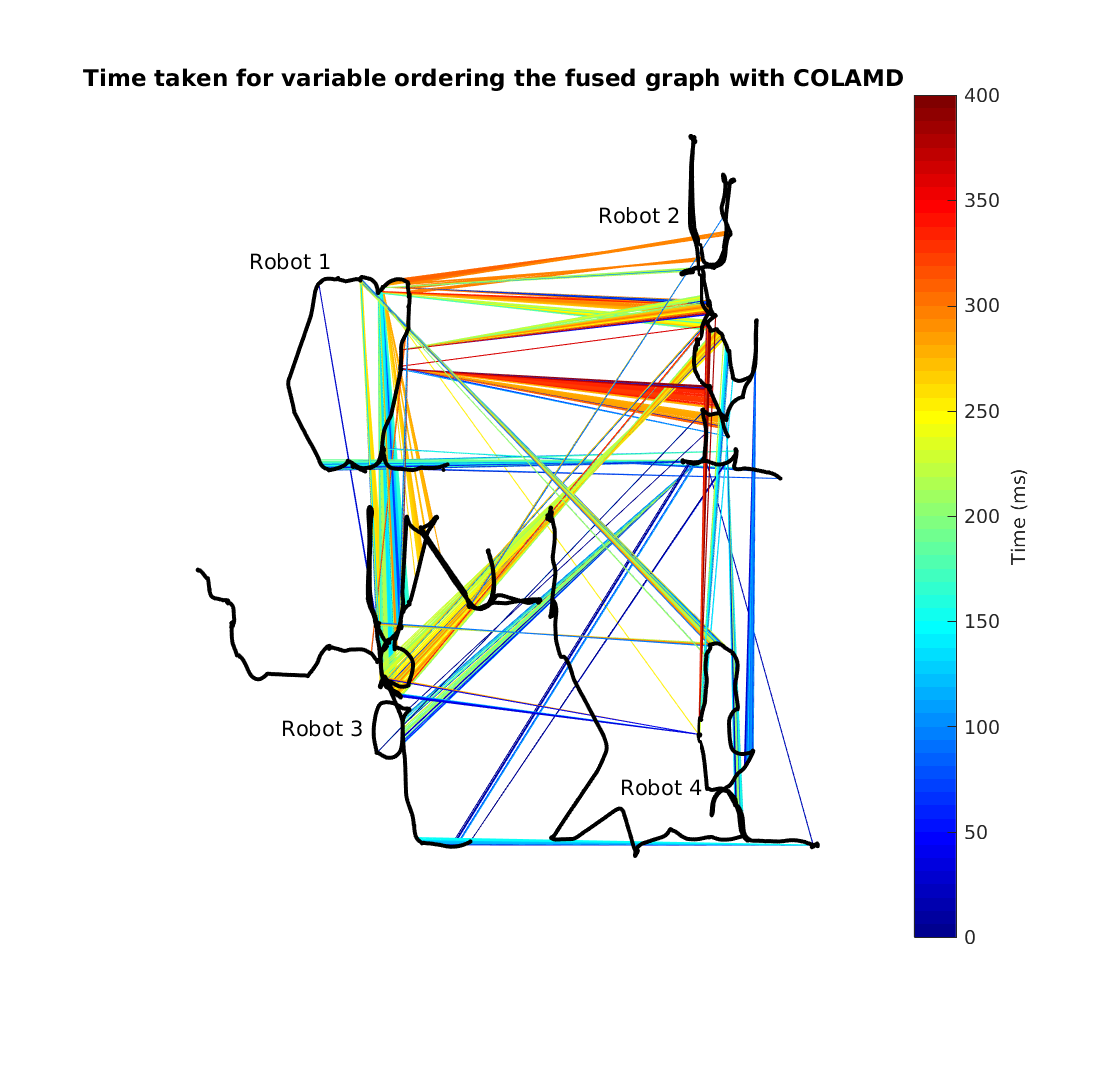
\includegraphics[width=\textwidth]{Chapters/figures6/colamd_ordering_encounter_colored}
\caption{The encounter map graphically describing the time taken for ordering the fused graph after every direct encounter using COLAMD \cite{colamd} ordering. The color of the line segment indicate the time taken and its endpoints indicate the poses corresponding to the encounter. A reference color bar is provided on the right. Note that the plot does not include indirect encounters as the trajectories are not in the original positioned and widely placed for clarity.}
\label{fig:encounter_colamd}
\end{figure}

\begin{figure}
\centering
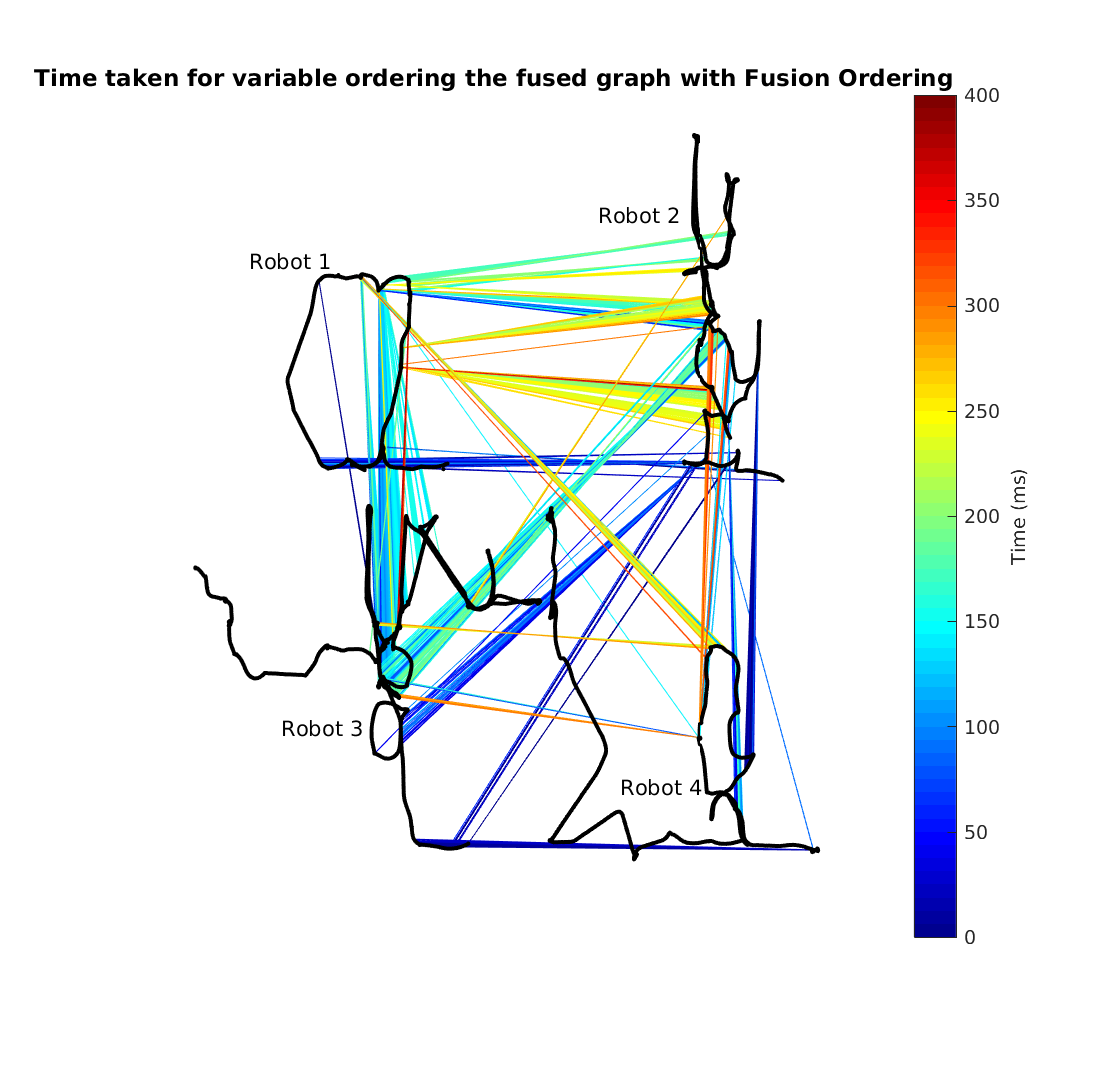
\includegraphics[width=\textwidth]{Chapters/figures6/fusion_ordering_encounter_colored}
\caption{The encounter map graphically describing the time taken for ordering the fused graph after every direct encounter using the proposed fusion ordering. The color of the line segment indicate the time taken and its endpoints indicate the poses corresponding to the encounter. A reference color bar is provided on the right. Note that the plot does not include indirect encounters as the trajectories are not in the original positioned and widely placed for clarity.}
\label{fig:encounter_fusion}
\end{figure}

\begin{figure}
\centering
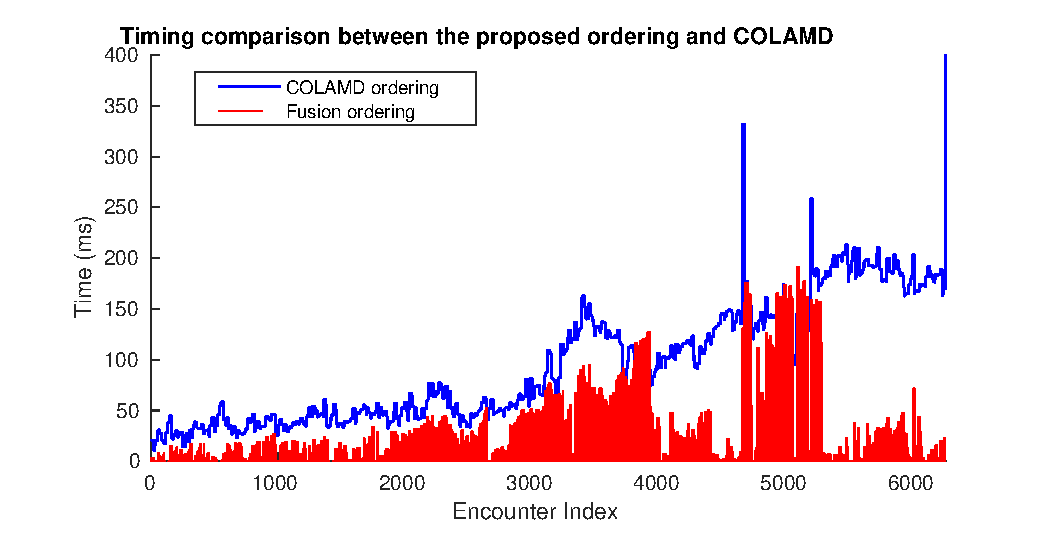
\includegraphics[width=\textwidth]{Chapters/figures6/time_fusion_vs_colamd}
\caption{Time comparison between the gold standard COLAMD and the proposed fusion ordering after every direct and indirect encounter. It can be observed that the time taken is lesser with fusion ordering for almost all the cases.}
\label{fig:fusion_vs_colamd}
\end{figure}

\section{Conclusions and Summary of Contributions}
In this thesis, we present a novel fusion ordering scheme for variable ordering the combination of multiple factor graphs using their parent ordering. We explain its relation with nested dissection to show the principle behind its working. A formal verification of the proposed algorithm is provided to ensure that it meets all the relevant standards and does not violate any canonical assumptions. One important aspect of the proposed algorithm is its potential to work in problems outside SLAM. Least squares is a standard approach for regression analysis and optimizing over-determined systems and is ubiquitous in engineering problems. Several factor graph applications in the field of finite element analysis, computational fluid dynamics and power network problem involve combining multiple graphs and variable ordering them for better estimation accuracy. We also presented a solution for relative pose graph initialization, a common problem in multi-robot mapping, that works within the framework of our problem formulation. The proposed factor type and the error function can be seamlessly added to the existing optimization problem and works for multiple and uncertain encounters with unknown data association. We demonstrate the results using standard real-world dataset from sparse linear algebra community called SuiteSparse and AP hill multi-robot dataset from radish repository. Introducing methods from the algebraic graph theory literature into the field of SLAM can be seen as another contribution. While several previous works have employed and innovated on matrix factorizations for SLAM, variable ordering the combined Jacobian from multiple robots has not been presented before. In particular, the combination of efficient fusion ordering, numerical stability ordering and relative pose graph initialization is novel and opens new possibilities that can be exploited in various robotics applications.

\section{Future Work}
Although the fusion ordering is quick and efficient in terms of time and storage, a thorough analysis about the change in the degree of the affected nodes in the fused graph with respect to the parent graph could be studied for different SLAM situations. This can lead to developing an upper bound on the additional number of non-zeros produced by using the fusion ordering instead of standard ordering techniques like COLAMD. Also, the structure of the ordered matrix coming out of fusion ordering is suitable for parallel QR decomposition according to \cite{parallelqr}, which I have not explored yet. The fusion ordering could be extended to work in the concurrent filtering and smoothing (CFS) framework \cite{cfs} for multiple robots. To get an end-to-end working real-time system it would interesting to investigate the bandwidth constraints in addition to the efficiency improvements proposed in this work. New factor types for encounters such as range-only or bearing-only might be studied in the context of relative pose graph initialization. 


